% FiLMVIB --- written internship report (15-30pp synthesis document).
%   Build:  cd paper && pdflatex report.tex && pdflatex report.tex   (twice, for the TOC/refs)
%
% Provenance rule, identical to final.tex and summary.tex: every value below is either (a) measured
% under our own evaluation protocol, or (b) reported by a cited publication with its arXiv identifier
% given where final.tex itself gives one. Nothing here is estimated or extrapolated. This document
% does not introduce any new empirical claim -- it restates, in full prose, exactly what paper/final.tex
% and paper/summary.tex already establish, expanded with the additional context and discussion a
% written report allows that slide bullets do not.
%
% Dependencies are the same minimal set already verified in this environment: geometry, xcolor,
% graphicx, tikz (positioning, arrows.meta), booktabs, amsmath, amssymb, lmodern/microtype (guarded),
% hyperref (guarded). No pgfplots (absent on the target machines; previously broke the build).

\documentclass[11pt,a4paper]{article}
\usepackage[a4paper,left=2.7cm,right=2.7cm,top=2.6cm,bottom=2.8cm]{geometry}
\usepackage{amsmath,amssymb}
\usepackage{booktabs}
\usepackage{xcolor}
\usepackage{graphicx}
\usepackage{tikz}
\usetikzlibrary{positioning,arrows.meta,calc}
\IfFileExists{lmodern.sty}{\usepackage{lmodern}}{}
\IfFileExists{microtype.sty}{\usepackage[protrusion=true,expansion=false]{microtype}}{}
\IfFileExists{hyperref.sty}{\usepackage[hidelinks,bookmarksnumbered]{hyperref}}{}

\graphicspath{{figures/}}
\definecolor{frz}{RGB}{40,95,175}     % frozen  (blue)
\definecolor{trn}{RGB}{210,120,20}    % trained (orange)
\definecolor{hdr}{RGB}{25,60,115}

\setlength{\parskip}{4pt}
\setlength{\parindent}{0pt}
\renewcommand{\arraystretch}{1.15}

% Figure slot that degrades to a labelled placeholder box if a file is absent, so the document
% always compiles -- same convention as final.tex and summary.tex.
\newcommand{\figslot}[2]{\IfFileExists{figures/#1}%
  {\includegraphics[width=#2]{figures/#1}}%
  {\fbox{\parbox[c][3cm][c]{#2}{\centering\small\ttfamily\detokenize{figures/#1}}}}}

\newcommand{\exlabel}[2]{{\small \color{red!65!black}base: #1 $\boldsymbol{\times}$\hspace{1em}%
  \color{green!40!black}ours: #2 $\boldsymbol{\checkmark}$}}

\title{\textbf{Making Frozen Audio--Visual LLMs Listen}\\[4pt]
  \large Audio Grounding via Tiny Adapters, Anchored Preference Optimization,\\ and Honest Evaluation\\[10pt]
  \normalsize\itshape Internship Report}
\author{Souleiman Sbai\\[4pt]
  \normalsize\normalfont \'Ecole Polytechnique\\
  Host laboratory: AIST CVRT \quad$\cdot$\quad Supervisor: Qiu Yue\\
  \texttt{souleiman.sbai@polytechnique.edu}}
\date{\today}

\begin{document}
\maketitle

\begin{abstract}
\noindent
Audio--visual large language models (LLMs) routinely answer questions about \emph{sound} using
\emph{visual} evidence instead: muting the audio track of Qwen3-Omni leaves its answers to
audio-existence questions unchanged, driving accuracy from 95.1\% to 0.0\%. This report presents
work carried out during a research internship investigating whether this failure can be repaired
\emph{without touching the backbone}. We attach a variational information bottleneck (VIB) to each
modality stream of a frozen audio--visual LLM ($<$0.5\% of backbone parameters, zero-initialized so
that it is exactly the identity map at attachment) and train it with an \emph{anchored} preference
objective on constructed audio--visual conflicts. Standard direct preference optimization (DPO) on
these pairs collapses to a constant response (perception accuracy $0.95\!\to\!0.10$); two explicit
constraints -- a chosen-answer anchor and a KL tether to the frozen backbone on ordinary inputs --
remove this degenerate optimum. On AVHBench ($n=5302$) the adapter improves overall accuracy by 5.1
points, and a query-conditioned (FiLM) variant by 5.8 points ($p<10^{-4}$, paired McNemar), while
preserving hallucination resistance and incurring no statistically significant cost on two
out-of-distribution capability controls (MMAU, Video-MME). Two independent probes separate the
underlying mechanisms: both variants increase the model's dependence on the audio stream by a factor
of 3.3--3.6, but only the query-conditioned variant also increases attention allocated to
audio--visual tokens. The method's reach is bounded by what the frozen backbone already encodes: the
gain is $+5.8$ points on Qwen3-Omni, $+0.1$ on Qwen2.5-Omni, and $-2.3$ on VideoLLaMA2 (whose audio
pathway was added post hoc); on temporal alignment, where the backbone is measured to be at chance
(0.495), no adapter helps. This report documents the method, the evaluation protocol designed to
test it honestly, the empirical results, the mechanistic analysis that explains them, and the
negative results and limitations that bound the claim.
\end{abstract}

\section*{Acknowledgements}
\noindent
I thank Qiu Yue and the AIST CVRT team for their supervision and for hosting this internship.
Computation was carried out on the ABCI cluster (group \texttt{gae50891}).

\tableofcontents
\clearpage

% ================================================================================================
\section{Introduction}
\label{sec:intro}

Audio--visual LLMs encode video and audio into token sequences, project each modality into the
language model's embedding space through a small adapter, and answer questions over the resulting
mixed sequence, in which text, audio, and vision tokens compete for the model's attention. This
architecture is now standard across a family of systems -- Qwen-Omni, VideoLLaMA, MiniCPM-O -- that
claim joint audio--visual understanding. In practice, these systems exhibit a systematic bias: when
a question can plausibly be answered from either modality, the answer tends to come from vision, even
when the correct answer requires the audio stream. Sung-Bin et al.\ (ICLR~2025) document this as
\emph{cross-modal hallucination} across every audio--visual LLM they evaluate, and Wen et al.\ (2026)
characterize it as a \emph{Clever Hans effect}: the model has learned to associate certain visual
scenes with certain sounds so reliably that it answers sound-related questions from visual priors
without consulting the audio stream at all. The clearest demonstration of this is an ablation
reported by Wen et al.\ on Qwen3-Omni, the backbone used throughout this work: muting the audio track
entirely leaves an ``is a sound audible'' question's accuracy essentially unchanged in \emph{direction}
-- it falls from 95.1\% to 0.0\%, meaning the model's answers stay consistent with what is visible,
not with what is (no longer) audible.

This report investigates a specific, narrow question: \textbf{can audio grounding in a frozen
audio--visual LLM be improved by training a parameter-efficient adapter alone}, without fine-tuning,
re-aligning, or otherwise modifying the backbone? The motivation for insisting on a frozen backbone
is threefold. First, it is the cheapest possible intervention: the adapter introduced here is
under 0.5\% of backbone parameters. Second, it is reversible: because the adapter is exactly the
identity map at initialization and can be bypassed at inference time, the original model is always
recoverable exactly. Third, it isolates the question of \emph{whether the necessary audio information
is already present in the frozen representation} from the question of whether the model can be taught
to use it -- a distinction that turns out to matter a great deal, as Section~\ref{sec:generalization}
shows.

The approach developed here has three components. A \textbf{variational information bottleneck}
(VIB) adapter is attached to each modality stream, trained with reparameterization and zero-initialized
so that attaching it changes nothing until training begins (Sections~\ref{sec:background}
and~\ref{sec:method}). An \textbf{anchored preference objective} is used in place of standard DPO,
which we show collapses to a degenerate, uniformly negative-answering solution on the audio-swap
training data used here; the anchored objective adds two explicit constraints that provably rule out
that degenerate optimum (Section~\ref{sec:method}). Finally, an \textbf{evaluation protocol} is
designed specifically to make the resulting accuracy numbers trustworthy: fixed decoding parameters,
held-out checkpoint selection, paired significance testing against the frozen baseline, three
independent capability controls, and evaluation across four different backbones
(Section~\ref{sec:setup}).

\subsection{Contributions}

This report makes the following contributions, each grounded in a measurement or a derivation
reported in the sections that follow:

\begin{itemize}
\item \textbf{C1.} A variational-bottleneck adapter, under 0.5\% of backbone parameters, that is
exactly the identity map at initialization and recovers the frozen backbone exactly when bypassed
(Section~\ref{sec:method}).
\item \textbf{C2.} An anchored preference objective that avoids the degenerate solution reached by
standard DPO on audio-swap data, using two explicit constraints derived from first principles
(Section~\ref{sec:method}).
\item \textbf{C3.} A query-conditioned (FiLM) variant of the adapter, together with mechanistic,
attention-based evidence distinguishing it from the unconditional variant (Sections~\ref{sec:method}
and~\ref{sec:mechanism}).
\item \textbf{C4.} An evaluation protocol with fixed decoding, held-out checkpoint selection, paired
significance testing, three capability controls, and four backbones (Section~\ref{sec:setup}).
\item \textbf{C5.} An extension of the same objective to temporal alignment, including new data
construction, a benchmark, and a measured (negative) baseline result that bounds what the method can
achieve (Section~\ref{sec:temporal}).
\end{itemize}

\subsection{Report Outline}

Section~\ref{sec:related} reviews the literature on cross-modal hallucination and situates this
work relative to existing mitigations. Section~\ref{sec:background} develops the mathematical
background of the variational information bottleneck that the adapter is built on, including a full
derivation of the tractable training objective. Section~\ref{sec:method} describes the adapter
architecture, the training-data construction, the failure mode of standard preference optimization
on this data, the anchored objective that repairs it, and the query-conditioned variant.
Section~\ref{sec:setup} describes the benchmarks and the experimental protocol.
Section~\ref{sec:results} reports the main results and their statistical significance, together with
two capability controls. Section~\ref{sec:mechanism} analyzes \emph{why} the method works, using
three independent probes. Section~\ref{sec:generalization} studies how the improvement scales across
four backbones and situates it relative to prior methods. Section~\ref{sec:temporal} reports a
negative result on temporal alignment that sharpens the method's boundary of applicability.
Section~\ref{sec:ablation} reports an architectural ablation and a table of negative results.
Section~\ref{sec:discussion} discusses limitations and reproducibility, and
Section~\ref{sec:conclusion} concludes.

\clearpage
% ================================================================================================
\section{Related Work}
\label{sec:related}

\subsection{Cross-Modal Hallucination in Audio--Visual LLMs}

\begin{figure}[h]
\centering
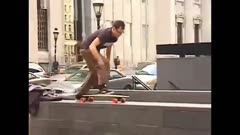
\includegraphics[width=0.30\linewidth]{avh_a2v_1.jpg}\hspace{2pt}%

\includegraphics[width=0.30\linewidth]{avh_a2v_2.jpg}\hspace{2pt}%
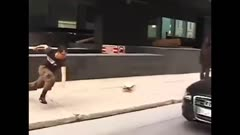
\includegraphics[width=0.30\linewidth]{avh_a2v_3.jpg}\\[4pt]

\includegraphics[width=0.30\linewidth]{avh_v2a_1.jpg}\hspace{2pt}%
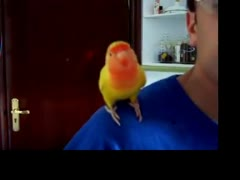
\includegraphics[width=0.30\linewidth]{avh_v2a_2.jpg}\hspace{2pt}%
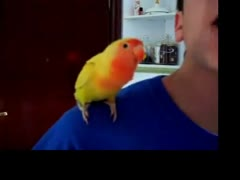
\includegraphics[width=0.30\linewidth]{avh_v2a_3.jpg}
\caption{Two AVHBench examples. \textbf{Top} (audio$\to$video): the audio contains a harsh grinding
sound; asked whether a power tool is visible, the frozen backbone answers ``yes'' (gold: ``no'').
\textbf{Bottom} (video$\to$audio): the clip is silent and shows a parrot on a shoulder; asked whether
the bird is making a sound, the frozen backbone again answers ``yes'' (gold: ``no'').}
\label{fig:problem}
\end{figure}

Figure~\ref{fig:problem} illustrates the phenomenon this work addresses with two concrete examples.
In the first, the audio track of a clip contains a harsh grinding sound; asked whether a power tool is
visible, the frozen backbone answers ``yes'' even though none is present -- the sound has induced a
visual hallucination. In the second, the video shows a parrot perched silently on a shoulder; asked
whether the bird is making a sound, the frozen backbone again answers ``yes,'' this time letting the
image induce an auditory hallucination in the opposite direction. Three independent lines of work
converge on the same diagnosis. \textbf{AVHBench} (Sung-Bin et al., ICLR~2025) introduces a
benchmark specifically designed to probe this failure and finds it present in every audio--visual LLM
evaluated. \textbf{CMM} (Leng et al., 2024) attributes the effect to an over-reliance on unimodal
priors learned during pretraining, and finds audio to be the modality most frequently overridden.
\textbf{Wen et al.\ (2026)} frame the phenomenon as a Clever Hans effect and quantify it directly on
Qwen3-Omni, the backbone used in this work, through three interventions summarized in
Table~\ref{tab:wen-interventions}: muting the audio track (an audio-existence probe), shifting it by
$\pm2$ seconds (a temporal-synchronization probe), and swapping it for another clip's audio (a
sound-consistency probe). All three interventions collapse accuracy far below what a model
genuinely attending to audio would be expected to show, with muting being the most severe: accuracy
falls to exactly zero, meaning every single response after muting remains consistent with the visual
content of the clip rather than reverting to a default or a chance-level distribution.

\begin{table}[h]
\centering
\small
\begin{tabular}{lccl}
\toprule
Probe & Original & Intervened & Intervention \\
\midrule
Audio existence   & 95.1  & \textcolor{red!70!black}{\textbf{0.0}}  & \emph{Mute}: silence the track \\
Temporal sync     & 100.0 & \textcolor{red!70!black}{\textbf{1.4}}  & \emph{Shift}: audio moved $\pm2$\,s \\
Sound consistency & 75.4  & \textcolor{red!70!black}{\textbf{37.3}} & \emph{Swap}: another clip's audio \\
\bottomrule
\end{tabular}
\caption{Wen et al.'s (2026) audio interventions on Qwen3-Omni, the backbone used throughout this
report (accuracy, \%). Reported values, arXiv:2605.16403, Table 1.}
\label{tab:wen-interventions}
\end{table}

\subsection{Existing Mitigations}

Three families of mitigation have been proposed. \textbf{Contrastive decoding} methods such as MAD
modify the decoding procedure to contrast predictions with and without the audio-visual conflict,
without retraining the model. \textbf{Modality-decoupled preference optimization} (MoD-DPO) fine-tunes
the full language model with a preference objective designed to decouple modality reliance.
\textbf{Full-model re-alignment} retrains the model end to end on curated data. All three modify or
bypass the frozen backbone in some way -- either by changing its weights or by changing its inference
procedure -- and none of them operates within the constraint explored in this report, namely that the
backbone itself is never touched, so its behaviour on any input outside the training distribution is
provably unchanged unless the adapter is active.

\subsection{Preference Optimization and Parameter-Efficient Fine-Tuning}

The training objective in this work builds on \textbf{Direct Preference Optimization} (DPO;
Rafailov et al., 2023), which reframes reinforcement learning from human feedback as a closed-form
classification loss over pairs of preferred and dispreferred responses, using the frozen (reference)
policy as an implicit reward baseline. Section~\ref{sec:method} shows that applying standard DPO
directly to the audio-swap data constructed for this project causes an identifiable failure mode
(likelihood displacement), motivating an anchor constraint in the style of \textbf{mDPO}
(Wang et al., 2024), which was originally proposed to prevent a related degeneracy in multimodal
preference optimization. On the architectural side, the adapter introduced here belongs to the family
of \textbf{parameter-efficient fine-tuning} methods, which train a small number of new parameters
while keeping a large pretrained model frozen. The most widely used member of this family,
\textbf{LoRA} (Hu et al., 2022), edits a frozen weight matrix with a low-rank additive correction.
The adapter used in this work is architecturally closer to the \textbf{bottleneck adapter} family
(Houlsby et al., 2019), which inserts a small module into the activation stream rather than editing a
weight matrix directly; Section~\ref{sec:ablation} reports a direct empirical comparison against LoRA
at matched attachment points.

\clearpage
% ================================================================================================
\section{Background: The Variational Information Bottleneck}
\label{sec:background}

The adapter developed in this work is built on the variational information bottleneck (VIB), a
tractable relaxation of the information bottleneck principle. This section develops the relevant
mathematics from first principles: Section~\ref{sec:ib-principle} states the (intractable) objective;
Section~\ref{sec:ib-bounds} derives the two variational bounds that make it tractable;
Section~\ref{sec:ib-reparam} derives the reparameterization trick used to train the resulting
objective by gradient descent, and the closed-form expression for its compression term that the
adapter's training loss uses directly.

\subsection{The Information Bottleneck Principle}
\label{sec:ib-principle}

The information bottleneck (Tishby et al., 2000) seeks a compressed representation $Z$ of an input
$X$ that retains only the information in $X$ that is predictive of a target $Y$. Formally, it seeks a
stochastic encoding $q(z\mid x)$ that solves
\begin{equation}
\max_{q(z\mid x)}\quad \underbrace{I(Z;Y)}_{\text{keep what predicts } Y} \;-\; \beta\, \underbrace{I(Z;X)}_{\text{forget the rest of } X},
\label{eq:ib}
\end{equation}
where $I(\cdot\,;\cdot)$ denotes mutual information and $\beta>0$ controls the trade-off between
retaining predictive information and discarding everything else. In this work, $X$ is a single
audio or video token as it leaves the frozen modality adapter, $Z$ is the corresponding bottlenecked
representation handed to the frozen language model, and $Y$ is the answer the language model must
produce. Equation~\eqref{eq:ib} is intractable as written, because both mutual-information terms
require distributions -- the true posterior $p(y\mid z)$ and the true marginal $p(z)$ -- that cannot
be computed in closed form for a stochastic encoder built from a neural network. The next section
derives a tractable surrogate.

\subsection{Two Variational Bounds}
\label{sec:ib-bounds}

Alemi et al.\ (ICLR~2017) show that Equation~\eqref{eq:ib} admits a tractable lower bound by
introducing two variational surrogates: a \emph{decoder} $q(y\mid z)$, approximating the true
$p(y\mid z)$, and a fixed \emph{prior} $r(z)$, approximating the true marginal $p(z)$. Both bounds
below follow from the same elementary fact, that Kullback--Leibler divergence is non-negative.

\paragraph{Relevance bound.} Writing $I(Z;Y)$ in terms of the entropy of $Y$,
\[
I(Z;Y) = H(Y) + \mathbb E_{p(x,y)}\mathbb E_{p(z\mid x)}\big[\log p(y\mid z)\big].
\]
For any $z$, $\mathrm{KL}\big(p(y\mid z)\,\|\,q(y\mid z)\big)\ge0$ is equivalent to
$\mathbb E_{p(y\mid z)}[\log p(y\mid z)] \ge \mathbb E_{p(y\mid z)}[\log q(y\mid z)]$, so substituting
$q(y\mid z)$ for the intractable $p(y\mid z)$ can only decrease the expression, giving a valid lower
bound:
\begin{equation}
I(Z;Y) \;\ge\; H(Y) + \mathbb E_{p(x,y)}\mathbb E_{p(z\mid x)}\big[\log q(y\mid z)\big].
\label{eq:relevance-bound}
\end{equation}
$H(Y)$ does not depend on the encoder or the decoder, so it is dropped from the training objective
without affecting what is being optimized; what remains, $\mathbb E[\log q(y\mid z)]$, is exactly a
\textbf{log-likelihood}. This is not incidental: it is the same quantity that reappears, evaluated at
the chosen and rejected candidate answers, as $c_p$ and $r_p$ in the DPO-style objective introduced in
Section~\ref{sec:method}. The decoder $q(y\mid z)$ in this work is literally the frozen language
model, decoding an answer conditioned on the adapter's bottlenecked output $z$.

\paragraph{Compression bound.} Writing $I(Z;X)$ in terms of the true marginal $p(z)=\int p(z\mid
x)p(x)\,dx$,
\[
I(Z;X) = \mathbb E_{p(x,z)}\big[\log p(z\mid x)\big] - \mathbb E_{p(z)}\big[\log p(z)\big].
\]
Because $\mathrm{KL}\big(p(z)\,\|\,r(z)\big)\ge0$ is equivalent to $\mathbb E_{p(z)}[\log p(z)] \ge
\mathbb E_{p(z)}[\log r(z)]$, substituting a fixed prior $r(z)$ for the intractable true marginal
$p(z)$ can only increase the expression being subtracted, giving a valid \emph{upper} bound:
\begin{equation}
I(Z;X) \;\le\; \mathbb E_{p(x)}\big[\mathrm{KL}\big(p(z\mid x)\,\|\,r(z)\big)\big].
\label{eq:compression-bound}
\end{equation}
In both cases, the bound is exact precisely when the chosen surrogate matches the true distribution
it stands in for: $q(y\mid z)=p(y\mid z)$ in the first case, $r(z)=p(z)$ in the second.

\paragraph{Combining the two bounds.} Because $\beta>0$ in Equation~\eqref{eq:ib}, upper-bounding the
term that is \emph{subtracted} still produces a lower bound on the difference: $-\beta I(Z;X) \ge
-\beta\,\mathbb E_x\big[\mathrm{KL}(p(z\mid x)\|r(z))\big]$. Both inequalities therefore point the
same way, and their sum is a certified lower bound on the true, intractable objective:
\begin{equation}
I(Z;Y) - \beta I(Z;X) \;\ge\;
\underbrace{\mathbb E\big[\log q(y\mid z)\big] \;-\; \beta\,\mathbb E_x\big[\mathrm{KL}(p(z\mid x)\|r(z))\big]}_{=:\ \mathcal R_{\text{VIB}}\ \text{(Alemi et al., ICLR 2017)}}.
\label{eq:rvib}
\end{equation}
Maximizing $\mathcal R_{\text{VIB}}$ by gradient ascent therefore maximizes a certified lower bound on
the true information-bottleneck objective, not merely a heuristic that resembles it. The first term
of $\mathcal R_{\text{VIB}}$ is a prediction loss (a log-likelihood); the second is a KL divergence to
a fixed prior, conventionally referred to as the \emph{rate}. $\beta$ corresponds to $\beta_{kl}$ in
the training objective used in this work (Section~\ref{sec:method}).

\subsection{Reparameterization and the Rate in Closed Form}
\label{sec:ib-reparam}

Maximizing $\mathcal R_{\text{VIB}}$ by gradient ascent requires $\nabla_\theta\,\mathbb
E_{p(z\mid x;\theta)}[f(z)]$ for some function $f$ (the log-likelihood, in the relevance term). This
gradient is not directly defined: $\theta$ names a \emph{distribution} that $z$ is sampled from, not
a value that a sampled point $z$ is a differentiable function of. Kingma and Welling (2014) resolve
this by rewriting the sampling step as a deterministic map of the input $x$ and \emph{parameter-free}
noise:
\begin{equation}
z = \mu(x) + \sigma(x)\odot\epsilon, \qquad \epsilon \sim \mathcal N(0,I).
\label{eq:reparam}
\end{equation}
For a fixed sample of $\epsilon$, $z$ is now an ordinary differentiable function of the encoder
outputs $\mu(x)$ and $\sigma(x)$, so $\nabla_\theta\,\mathbb E_\epsilon[f(z)] = \mathbb
E_\epsilon[\nabla_\theta f(z)]$: a single Monte Carlo sample of $\epsilon$ gives an unbiased gradient
estimator. This is exactly the encoder used in the adapter architecture described in
Section~\ref{sec:method}.

The compression term of $\mathcal R_{\text{VIB}}$ needs no such Monte Carlo estimate at all. With
$q(z\mid x)=\mathcal N(\mu,\sigma^2 I)$ (the encoder's own output distribution) and $r(z)=\mathcal
N(0,I)$ (a fixed, standard-normal prior), both Gaussian, the KL divergence has a closed form. For a
single coordinate, using $\mathbb E_q[(z-\mu)^2]=\sigma^2$ and $\mathbb E_q[z^2]=\sigma^2+\mu^2$,
\[
\mathrm{KL}\big(\mathcal N(\mu,\sigma^2)\,\|\,\mathcal N(0,1)\big)
= -\log\sigma - \tfrac12 + \tfrac{\sigma^2+\mu^2}{2}
= \tfrac12\big(\mu^2+\sigma^2-1-\log\sigma^2\big).
\]
Summing over the $d$ coordinates of the latent $z$ gives the rate used throughout this work:
\begin{equation}
\mathrm{KL}\big(\mathcal N(\mu,\sigma^2I)\,\|\,\mathcal N(0,I)\big)
= \tfrac12 \sum_{i=1}^{d} \big(\mu_i^2 + \sigma_i^2 - 1 - \log\sigma_i^2\big).
\label{eq:kl-closed-form}
\end{equation}
This is exactly the quantity referred to as $\mathrm{KL}_{\text{VIB}}$ in the anchored objective of
Section~\ref{sec:method}: a closed-form penalty computed directly from the encoder's own $\mu(x)$ and
$\sigma(x)$ outputs, requiring no sampling for this half of the bound.

\clearpage
% ================================================================================================
\section{Method}
\label{sec:method}

\subsection{Bottleneck Architecture}
\label{sec:arch}

\begin{figure}[h]
\centering
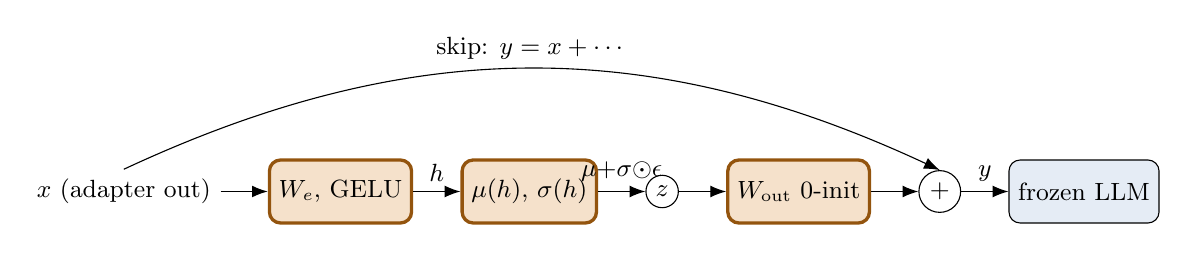
\begin{tikzpicture}[font=\small,>={Latex[length=2mm]},node distance=3mm and 6mm,
  trn/.style={draw,very thick,rounded corners,fill=trn!22,draw=trn!70!black,minimum height=8mm,align=center},
  frzs/.style={draw,rounded corners,fill=frz!12,minimum height=8mm,align=center},
  op/.style={draw,circle,inner sep=2pt},
  io/.style={align=center}]
  \node[io] (x) {$x$ \small(adapter out)};
  \node[trn,right=of x] (enc) {$W_e$, GELU};
  \node[trn,right=of enc] (ms) {$\mu(h),\,\sigma(h)$};
  \node[op,right=of ms] (z) {$z$};
  \node[trn,right=of z] (wout) {$W_{\text{out}}$ \small 0-init};
  \node[op,right=of wout] (add) {$+$};
  \node[frzs,right=of add] (llm) {frozen LLM};
  \draw[->] (x)--(enc); \draw[->] (enc)--node[above]{\small $h$}(ms);
  \draw[->] (ms)--node[above]{\small $\mu{+}\sigma{\odot}\epsilon$}(z);
  \draw[->] (z)--(wout); \draw[->] (wout)--(add);
  \draw[->] (add)--node[above]{\small $y$}(llm);
  \draw[->] (x.north) to[out=25,in=155] node[above,pos=0.5]{\small skip: $y=x+\cdots$} (add.north);
\end{tikzpicture}
\caption{The variational bottleneck attached to each modality stream. Blue nodes are frozen; orange
nodes are trained. $x$ is the token as it leaves the frozen modality adapter; $y$ is what the frozen
LLM actually receives.}
\label{fig:arch}
\end{figure}

Figure~\ref{fig:arch} shows the adapter attached to each modality stream. Given a token $x$ as it
leaves the frozen modality adapter, a small trained encoder $W_e$ followed by a GELU nonlinearity
produces a hidden representation $h$, from which two linear heads produce the parameters $\mu(h)$ and
$\sigma(h)$ of a diagonal Gaussian. The latent $z$ is drawn using the reparameterization of
Equation~\eqref{eq:reparam}, and a trained output projection $W_{\text{out}}$ maps it back into the
token space as a residual correction:
\begin{equation}
z = \mu(x) + \sigma(x)\odot\epsilon, \qquad y = x + W_{\text{out}}\,z, \qquad
W_{\text{out}} \stackrel{\text{init}}{=} 0.
\label{eq:bottleneck}
\end{equation}
Two properties of this construction matter for what follows. First, because $W_{\text{out}}$ is
zero-initialized, $y=x$ identically at initialization: attaching the module to the frozen backbone
provably changes nothing about its behaviour until training begins. Second, a bypass flag recovers
the frozen backbone \emph{exactly} by skipping the bottleneck entirely, which supplies the reference
distribution needed for the preference objective of Section~\ref{sec:objective} without
instantiating a second copy of the model. One such module is attached per modality (audio and
vision); together, the two modules are under 0.5\% of backbone parameters.

\subsection{Training Data: Constructed Audio--Visual Conflicts}
\label{sec:data}

\begin{figure}[h]
\centering
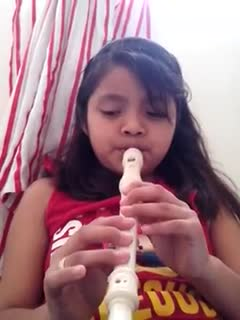
\includegraphics[width=0.42\linewidth]{as_flute_1.jpg}\hspace{2pt}%

\includegraphics[width=0.42\linewidth]{as_flute_2.jpg}
\caption{Two frames from a training example constructed by overlaying a different clip's audio onto
a silent recorder-playing video: the visible event is a flute, the (overlaid) audible event is a
train horn. Asked which event is heard, the frozen backbone answers ``flute'' (the visible event); the
adapted model answers ``train horn'' (the audible event).}
\label{fig:flute}
\end{figure}

The adapter must be trained on instances where relying on vision alone produces a wrong answer,
otherwise there is no training signal that specifically targets audio grounding. Such instances are
constructed directly: given a clip, its audio track is substituted for a different clip's audio
track drawn from a different event category, so that the visible and audible events disagree. In the
example shown in Figure~\ref{fig:flute}, the video shows a child playing a flute (a recorder); the
audio is replaced with a train horn. Preferring the audio-consistent answer -- ``train horn'' -- on
such an instance is only possible by actually using the audio stream, since every visual cue in the
clip points to the flute.

\subsection{The Failure Mode of Standard Preference Optimization}
\label{sec:dpo-fails}

Given a chosen (audio-consistent) and a rejected (vision-consistent) answer for each constructed
conflict, the natural training objective is Direct Preference Optimization (Rafailov et al., 2023).
Writing $c$ and $r$ for the log-probability of the chosen and rejected answer respectively, and
subscript $p$ for ``adapter on'' and subscript $r$ for ``adapter bypassed'' (the frozen base, which
serves as the reference policy for free, by Section~\ref{sec:arch}'s bypass property), the standard
DPO loss is
\begin{equation}
\mathcal L_{\text{DPO}} = -\log\sigma\Big(\beta\big[(c_p-c_r) - (r_p-r_r)\big]\Big), \qquad \beta=0.1,
\label{eq:dpo}
\end{equation}
where $\sigma$ is the logistic sigmoid (not to be confused with the encoder's standard deviation
$\sigma(x)$), and $\beta$ here is the DPO temperature (not to be confused with the VIB rate
$\beta_{kl}$ of Section~\ref{sec:background}; this notational collision is unfortunate but standard
in both literatures, and is flagged explicitly wherever it could cause ambiguity in this report).
Equation~\eqref{eq:dpo} constrains only the \emph{margin} between the chosen and rejected candidates:
it is minimized even when both $c_p$ and $r_p$ decrease, provided the rejected candidate's
probability decreases faster. In practice, this means the loss can be driven to zero while both
answers' probabilities collapse and the freed probability mass accumulates on a third,
unconstrained response -- a phenomenon known as \emph{likelihood displacement}. Training with
Equation~\eqref{eq:dpo} directly on the constructed conflicts of Section~\ref{sec:data} reduces
perception accuracy (as measured by the CMM benchmark of Section~\ref{sec:setup}) from 0.95 to 0.10:
the model converges to answering ``no'' for essentially every input, regardless of whether a
described object or sound is actually present. Because this degenerate solution attains maximal
hallucination resistance under CMM (a model that never says ``yes'' is never caught hallucinating a
positive), a hallucination-resistance metric evaluated in isolation would report this collapse as an
improvement. This is why Section~\ref{sec:setup} insists that perception accuracy and hallucination
resistance be reported jointly, and it is the central empirical motivation for the anchored objective
introduced next.

\subsection{Anchored Objective}
\label{sec:objective}

The anchored objective adds two explicit constraints to the DPO engine of Equation~\eqref{eq:dpo},
each targeting one half of the degenerate solution identified above:
\begin{align}
\mathcal L =\ & \underbrace{-\log\sigma\big(\beta[(c_p{-}c_r){-}(r_p{-}r_r)]\big)}_{\text{engine: prefer the heard answer}}
 \;+\; \lambda_a\,\underbrace{\big({-}\log\sigma(\beta(c_p{-}c_r){-}\delta)\big)}_{\text{rail 1: chosen} \ge \text{base} \Rightarrow \text{PA}} \nonumber\\[2pt]
 &+\; \lambda_{kl}\,\underbrace{\mathrm{KL}\!\big(p_{\text{base}}\,\|\,p_\theta\big)}_{\text{rail 2: normal inputs unchanged} \Rightarrow \text{HR}}
 \;+\; \beta_{kl}\,\mathrm{KL}_{\text{VIB}}.
\label{eq:anchored}
\end{align}
\textbf{Rail 1} is an mDPO-style anchor (Wang et al., 2024): it directly penalizes any drop in the
chosen response's probability relative to the frozen backbone, which is exactly what would happen if
training pushed both candidate probabilities down together. \textbf{Rail 2} penalizes divergence
from the frozen backbone's output distribution on ordinary, non-substituted inputs, which is exactly
what preserves capability on inputs the training data never touches. The uniform-``no'' solution of
Section~\ref{sec:dpo-fails} violates both constraints simultaneously -- it lowers the chosen
response's probability (violating rail 1) and changes behaviour on ordinary inputs (violating rail 2)
-- so the preference term can only be reduced by genuinely using the audio stream to distinguish
chosen from rejected answers. The final term, $\beta_{kl}\,\mathrm{KL}_{\text{VIB}}$, is exactly the
closed-form rate of Equation~\eqref{eq:kl-closed-form}, applied to both modality bottlenecks.

\subsection{Query-Conditioned Variant (FiLM)}
\label{sec:film}

\begin{figure}[h]
\centering
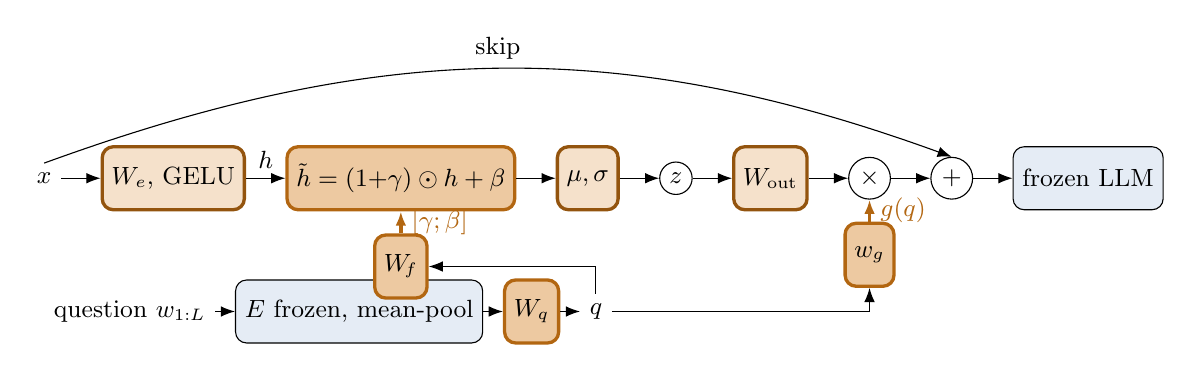
\begin{tikzpicture}[font=\small,>={Latex[length=1.8mm]},node distance=3mm and 5mm,
  trn/.style={draw,very thick,rounded corners,fill=trn!22,draw=trn!70!black,minimum height=8mm,align=center},
  new/.style={draw,very thick,rounded corners,fill=trn!40,draw=trn!85!black,minimum height=8mm,align=center},
  frzs/.style={draw,rounded corners,fill=frz!12,minimum height=8mm,align=center},
  op/.style={draw,circle,inner sep=2pt},
  io/.style={align=center}]
  \node[io] (x) {$x$};
  \node[trn,right=of x] (enc) {$W_e$, GELU};
  \node[new,right=of enc] (film) {$\tilde h=(1{+}\gamma)\odot h+\beta$};
  \node[trn,right=of film] (ms) {$\mu,\sigma$};
  \node[op,right=of ms] (z) {$z$};
  \node[trn,right=of z] (wout) {$W_{\text{out}}$};
  \node[op,right=of wout] (mult) {$\times$};
  \node[op,right=of mult] (add) {$+$};
  \node[frzs,right=of add] (llm) {frozen LLM};
  \draw[->] (x)--(enc); \draw[->] (enc)--node[above]{\small $h$}(film);
  \draw[->] (film)--(ms); \draw[->] (ms)--(z);
  \draw[->] (z)--(wout); \draw[->] (wout)--(mult); \draw[->] (mult)--(add);
  \draw[->] (add)--(llm);
  \draw[->] (x.north) to[out=20,in=160] node[above,pos=0.5]{\small skip} (add.north);
  \node[io,below=15mm of x,anchor=west] (w) {question $w_{1:L}$};
  \node[frzs,right=2.5mm of w] (embed) {$E$ frozen, mean-pool};
  \node[new,right=2.5mm of embed] (wq) {$W_q$};
  \node[io,right=2.5mm of wq] (qv) {$q$};
  \node[new] (wf) at ([yshift=-7mm]film.south) {$W_{\!f}$};
  \node[new] (wg) at ([yshift=-7mm]mult.south) {$w_g$};
  \draw[->] (w)--(embed); \draw[->] (embed)--(wq); \draw[->] (wq)--(qv);
  \draw[->] (qv.north) |- (wf.east);
  \draw[->] (qv.east) -| (wg.south);
  \draw[->,trn!85!black,very thick] (wf.north)--node[right]{\small $[\gamma;\beta]$}(film.south);
  \draw[->,trn!85!black,very thick] (wg.north)--node[right]{\small $g(q)$}(mult.south);
\end{tikzpicture}
\caption{The query-conditioned (FiLM) variant. The main path (left) is the plain VIB of
Figure~\ref{fig:arch}; the question path (bottom) pools a frozen embedding of the question into $q$,
which produces a per-feature scale/shift $[\gamma;\beta]$ applied before the bottleneck and a scalar
gate $g(q)$ applied after it. $\gamma,\beta$ here are FiLM's own scale and shift parameters (Perez et
al., 2018) -- unrelated to the DPO temperature $\beta$ or the VIB rate $\beta_{kl}$.}
\label{fig:film}
\end{figure}

The unconditional adapter of Section~\ref{sec:arch} processes every token identically, regardless of
what the current question is asking about. Section~\ref{sec:loss-floor} shows this is provably
insufficient on part of the constructed training data. The query-conditioned variant, illustrated in
Figure~\ref{fig:film}, extends the architecture using Feature-wise Linear Modulation (FiLM; Perez et
al., 2018): a frozen, mean-pooled embedding of the question text is projected into a vector $q$,
which is in turn used to produce a per-feature scale and shift $[\gamma;\beta]$ applied to the
encoder's hidden state before the bottleneck, and a scalar gate $g(q)\in(0,1)$ applied to the
bottleneck's output before it is added back to the residual stream. All newly introduced weights
($W_q$, $W_f$, $w_g$) are small linear heads; the frozen embedding table $E$ and the mean-pooling
operation introduce no new parameters. As in the unconditional case, $W_{\text{out}}$ remains
zero-initialized, so the variant is still exactly the identity map at initialization.

\subsection{Why Query Conditioning Is Necessary: A Loss-Floor Argument}
\label{sec:loss-floor}

\begin{table}[h]
\centering
\small
\renewcommand{\arraystretch}{1.25}
\begin{tabular}{llccc}
\toprule
Adapter & Answers (hear / see) & Hear loss & See loss & Total \\
\midrule
Cannot read $q$, commits to ``bell'' & ``bell'' / ``bell'' & $0.13$ & $2.13$ & $2.26$ \\
Cannot read $q$, hedges 50/50        & --- & $0.69$ & $0.69$ & $\mathbf{1.39}$ (floor) \\
\textbf{Reads $q$}                   & ``bell'' / ``dog''  & $0.13$ & $0.13$ & $\mathbf{0.26\to 0}$ \\
\bottomrule
\end{tabular}
\caption{A query-independent adapter cannot beat a loss floor of $2\log2\approx1.39$ per pair; a
query-conditioned one can drive the loss to zero.}
\label{tab:loss-floor}
\end{table}

This subsection gives a short argument, independent of any experiment, for why query conditioning is
necessary at the optimum of the training objective, not merely a convenient extension. Consider one
substituted clip in which the visible event is a dog and the (overlaid) audible event is a bell, and
two questions posed over the identical input: ``what do you hear?'' (correct answer: bell) and ``what
do you see?'' (correct answer: dog). Writing the per-question loss as $-\log\sigma(m)$ for margin
$m$, the values $m=+2,0,-2$ give losses of $0.13$, $0.69$, and $2.13$ respectively. Table
\ref{tab:loss-floor} works through the three possible strategies available to an adapter that cannot
condition on the question text: it can commit to one answer for both questions, hedge 50/50 between
them, or -- the only remaining option -- read the question and answer each correctly. Committing to a
single answer incurs the full margin-loss penalty on whichever question it gets wrong; hedging
incurs the intermediate loss $-\log\sigma(0)=\log2$ on both questions, for a floor of $2\log2\approx
1.39$ per pair that no query-independent strategy can beat. A query-conditioned adapter, by contrast,
can answer both questions correctly and drive the loss to exactly zero. Because the training data of
Section~\ref{sec:data} contains exactly this kind of paired question over a single substituted clip,
the data construction makes query conditioning necessary at the optimum of the objective -- a
property of the objective itself, established here independently of any training run.

\clearpage
% ================================================================================================
\section{Experimental Setup}
\label{sec:setup}

\subsection{Benchmarks}
\label{sec:benchmarks}

Five benchmarks are used in this work, each measuring a different aspect of the method's behaviour.

\paragraph{AVHBench.} The primary hallucination benchmark (Sung-Bin et al., ICLR 2025) comprises
5,302 yes/no questions over 2,136 videos, summarized in Table~\ref{tab:avhbench}. Three judgment
tasks are distinguished: \textbf{A$\to$V}, whether a queried object is visible, where the audible
event can induce false positives; \textbf{V$\to$A}, whether a queried sound is audible, where the
visible event can induce false positives, and which serves as this work's primary measure of audio
grounding; and \textbf{A--V Matching}, whether the audio and video correspond, which requires
integrating both modalities. Labels are exactly balanced within each task, so a constant response
yields 50\% accuracy.

\begin{table}[h]
\centering
\small
\begin{tabular}{lrrr}
\toprule
Judgment task & QnA & Yes & No \\
\midrule
A$\to$V (audio$\to$video) & 1,136 & 568 & 568 \\
V$\to$A (video$\to$audio) & 2,290 & 1,145 & 1,145 \\
A--V Matching             & 1,876 & 938 & 938 \\
\midrule
\textbf{Total}            & \textbf{5,302} & 2,651 & 2,651 \\
\bottomrule
\end{tabular}
\caption{AVHBench composition (Sung-Bin et al., ICLR 2025): 2,136 videos, 5,302 questions.}
\label{tab:avhbench}
\end{table}

\paragraph{CMM.} The capability benchmark (Leng et al., 2024) comprises 1,200 samples, each probed
with two questions -- one about an object present in the clip (gold answer ``yes''), one about an
absent object (gold answer ``no'') -- for 2,400 questions total. Perception accuracy (PA) and
hallucination resistance (HR) are defined as
\[
\mathrm{PA} = \frac{\#\text{ correct ``yes''}}{\#\text{ ground-truth ``yes''}}, \qquad
\mathrm{HR} = \frac{\#\text{ correct ``no''}}{\#\text{ ground-truth ``no''}}.
\]
These two metrics must always be reported jointly: a model that answers ``no'' unconditionally
attains $\mathrm{HR}=1.0$ and $\mathrm{PA}=0$, so an improvement in hallucination resistance is
only meaningful when it is not purchased at the cost of perception accuracy. As
Section~\ref{sec:dpo-fails} shows, this is not a hypothetical concern.

\paragraph{MMAU and Video-MME.} Two further benchmarks serve as out-of-distribution capability
controls, described in full in Section~\ref{sec:capability}: MMAU ($n=1000$) probes general
audio-only reasoning across sound, music, and speech categories, with no visual component; Video-MME
($n=900$, short subset, no subtitles) probes general video question answering. Neither benchmark
involves the audio--visual conflicts the adapter is trained on, so both serve as a check that the
adapter's training has not degraded capability more broadly.

\paragraph{AVE-Shift.} A benchmark constructed for this work specifically to probe temporal alignment
(Section~\ref{sec:temporal}), built by displacing a clip's audio track by a controlled offset and
asking the model to judge whether audio and video are synchronized.

\subsection{Protocol}
\label{sec:protocol}

Five aspects of the evaluation protocol were fixed in advance and are reported here because each was
found, during this project, to materially affect the reported numbers.

\begin{itemize}
\item \textbf{Frame rate} is fixed in code at 2\,fps for Qwen3-Omni (1\,fps for the smaller 7B
backbones), identically for checkpoint selection and final evaluation. Below 2\,fps, Qwen3-Omni was
found to exhibit a systematic bias toward affirmative answers, which would otherwise confound any
comparison across configurations that did not hold frame rate fixed.
\item \textbf{Prompt sensitivity is substantial.} Altering only the answer-format suffix of the
prompt -- with identical model weights -- changed one score by 11 points (V$\to$A, from 69.0 to
80.3). Prompts, the answer-format suffix, and all decoding parameters are therefore fixed for every
row of every table in this report and logged alongside the corresponding results.
\item \textbf{Checkpoint selection} is performed on a validation half of each benchmark, with results
reported on the disjoint remainder. This distinction mattered in practice: the checkpoint initially
selected during development did not survive this held-out evaluation procedure and was replaced.
\item \textbf{Significance testing} is paired: because the frozen baseline and every trained variant
are evaluated on identical items, McNemar's test with bootstrap confidence intervals is used rather
than treating the two accuracies as independent samples (Section~\ref{sec:significance}).
\item \textbf{Contamination} between the constructed training data and every benchmark used for
evaluation was checked by script; the intersection of training and benchmark clips is empty in every
case reported here.
\end{itemize}

Reported accuracies throughout this report are meaningful only relative to this fixed protocol; they
should not be compared to numbers reported elsewhere under different decoding or prompting choices
without accounting for the sensitivity documented above. Section~\ref{sec:minicpm} returns to this
point with a direct, quantified example.

\clearpage
% ================================================================================================
\section{Results}
\label{sec:results}

\subsection{Main Results}
\label{sec:main-results}

\begin{table}[h]
\centering
\small
\renewcommand{\arraystretch}{1.2}
\begin{tabular}{lccccccc}
\toprule
& \multicolumn{4}{c}{AVHBench ($n=5302$)} & \multicolumn{3}{c}{CMM ($n=2400$)} \\
\cmidrule(lr){2-5}\cmidrule(lr){6-8}
 & A$\to$V & V$\to$A & AV-m & Overall & PA & HR & Overall \\
\midrule
Gemini (closed) & 0.850 & 0.747 & 0.603 & 0.718 & 0.907 & 0.628 & 0.768 \\
GPT-4o (closed) & 0.846 & 0.510 & 0.501 & 0.579 & 0.359 & 0.892 & 0.626 \\
\midrule
Frozen base                    & \textbf{0.838} & 0.812 & 0.653 & 0.761 & \textbf{0.900} & 0.733 & 0.816 \\
$+$ cross-attention (step 60)  & \textbf{0.850} & 0.805 & 0.696 & 0.776 & \multicolumn{3}{c}{\emph{CMM running}} \\
$+$ LoRA $r{=}16$ (step 90)    & 0.828 & 0.835 & 0.709 & 0.789 & 0.896 & 0.724 & 0.810 \\
$+$ swap-DPO (step 60)         & 0.837 & \textbf{0.838} & 0.766 & 0.812 & 0.890 & 0.743 & 0.816 \\
$+$ \textbf{FiLM} (step 160)   & 0.822 & 0.827 & \textbf{0.808} & \textbf{0.819} & 0.894 & \textbf{0.746} & \textbf{0.820} \\
\bottomrule
\end{tabular}
\caption{Main results on Qwen3-Omni, full benchmarks. All rows evaluated under the fixed protocol of
Section~\ref{sec:protocol}; adapters selected on a validation half.}
\label{tab:main-results}
\end{table}

Table~\ref{tab:main-results} reports the central empirical result of this work. Both proposed
adapters improve AVHBench overall accuracy relative to the frozen base -- by 5.1 points for the
unconditional swap-DPO variant and 5.8 points for the query-conditioned FiLM variant -- while
preserving CMM capability: hallucination resistance increases in both cases, and perception accuracy
decreases by at most one point, in sharp contrast to the collapse documented in
Section~\ref{sec:dpo-fails}. The improvement is not distributed uniformly across AVHBench's three
tasks: it is concentrated in A--V Matching, which improves from 0.653 to 0.808 (+15.5 points),
consistent with this being the task that most directly requires integrating both modalities rather
than answering from either one alone. For context, Table~\ref{tab:main-results} also reports two
closed, general-purpose multimodal models evaluated under the same protocol. GPT-4o's combination of
$\mathrm{HR}=0.892$ with $\mathrm{PA}=0.359$ is a real-world instance of the degenerate solution
described in Section~\ref{sec:dpo-fails}, occurring in a deployed system rather than a
failed training run.

\subsection{Statistical Significance}
\label{sec:significance}

\begin{table}[h]
\centering
\small
\begin{tabular}{lccl}
\toprule
Comparison (held-out) & $b$ / $c$ & $\Delta$ [95\% CI] & Verdict \\
\midrule
Base $\to$ swap-DPO & 152 / 411 & $+5.2$ [+4.3, +6.1] & Real ($p<10^{-4}$) \\
Base $\to$ FiLM     & 253 / 532 & $+5.6$ [+4.5, +6.7] & Real ($p<10^{-4}$) \\
DPO $\to$ FiLM      & 204 / 224 & $+0.4$ [-0.4, +1.2] & Tie; FiLM wins AV-m ($+3.7$, $p<10^{-4}$) \\
\bottomrule
\end{tabular}
\caption{Paired significance analysis. $b$: items answered correctly by the baseline alone; $c$: by
the adapted model alone; $\Delta=(c-b)/N$.}
\label{tab:significance}
\end{table}

Because the baseline and every trained variant are evaluated on identical items, only discordant
pairs are informative: of $N$ items, $b$ are answered correctly by the baseline alone and $c$ by the
adapted model alone, giving
\[
\Delta = \frac{c-b}{N}, \qquad
\text{95\% CI: } \Delta \pm 1.96\,\frac{\sqrt{(b+c)-(c-b)^2/N}}{N}, \qquad
\text{McNemar's test: is } b/c \text{ a fair coin?}
\]
Table~\ref{tab:significance} reports this analysis on the held-out evaluation split. The discordant
counts for both proposed adapters (411 versus 152 for swap-DPO; 532 versus 253 for FiLM) are
strongly inconsistent with an equal-probability null, confirming that the improvements reported in
Table~\ref{tab:main-results} are real rather than an artefact of item sampling. The direct comparison
between the two proposed variants is a statistical tie on overall accuracy, though FiLM wins
specifically on A--V Matching. These results are from a single training seed in each case; the
reported intervals reflect item-sampling uncertainty only, and do not capture variation across
training seeds, which Section~\ref{sec:limitations} lists among the study's limitations.

\subsection{Capability Controls}
\label{sec:capability}

Two further benchmarks, unrelated to the audio--visual conflicts used in training, bound the cost of
the intervention on general capability.

\begin{table}[h]
\centering
\small
\begin{tabular}{lcccc}
\toprule
Qwen3-Omni & Sound & Music & Speech & Avg. \\
\midrule
Frozen base    & \textbf{80.2} & \textbf{75.4} & \textbf{68.5} & \textbf{74.7} \\
$+$ swap-DPO   & 78.4 & 75.1 & 67.0 & 73.5 \\
$+$ FiLM       & 79.6 & 73.1 & 66.4 & 73.0 \\
\bottomrule
\end{tabular}
\caption{Capability control I: MMAU, general audio understanding ($n=1000$, parse rate 0.94 on all
rows).}
\label{tab:mmau}
\end{table}

Table~\ref{tab:mmau} reports MMAU, which probes audio-only reasoning with no video and no
hallucination-inducing construction, and is therefore out of distribution for this method. Both
adapters incur a small cost: $-1.2$ points for swap-DPO, $-1.7$ for FiLM. Both differences lie within
the $\pm2.8$-point interval expected from sampling noise at $n=1000$, but the sign is consistently
negative and is reported as such rather than rounded to ``no effect.'' The natural reading is that
learning \emph{which} modality to trust on constructed conflicts does not transfer to general audio
understanding.

\begin{table}[h]
\centering
\small
\begin{tabular}{lcc}
\toprule
Qwen3-Omni & Accuracy & $\Delta$ \\
\midrule
Frozen base  & \textbf{0.842} & --- \\
$+$ swap-DPO & 0.828 & $-1.4$ \\
$+$ FiLM     & 0.837 & $-0.6$ \\
\bottomrule
\end{tabular}
\caption{Capability control II: Video-MME, general video understanding ($n=900$, short subset,
without subtitles).}
\label{tab:videomme}
\end{table}

Table~\ref{tab:videomme} reports Video-MME under the same pinned harness (900 YouTube videos, three
multiple-choice questions each; short subset; audio taken from the video itself). The 95\% interval
at this sample size is $\pm2.4$ points, so both differences are statistically indistinguishable from
zero, indicating no significant loss of general video question-answering capability. The ordering
between the two adapters matches MMAU -- FiLM preserves capability better than swap-DPO on both
controls -- which is consistent with the mechanistic distinction developed in
Section~\ref{sec:mechanism}. Taken together, the three controls in this report show a consistent
pattern: hallucination resistance on CMM improves, while audio and video understanding on MMAU and
Video-MME show small, non-significant decreases. The improvement is specific to the training
distribution, and its cost elsewhere is quantified here rather than assumed away.

\clearpage
% ================================================================================================
\section{Mechanism Analysis}
\label{sec:mechanism}

Table~\ref{tab:main-results} shows that both proposed adapters achieve a comparable improvement in
accuracy. This section asks whether they achieve it the same way, using three independent probes,
none of which was used during training or model selection.

\subsection{Attention to Audio--Visual Tokens}
\label{sec:attention}

\begin{figure}[h]
\centering
\figslot{attn_av.png}{0.62\linewidth}
\caption{Share of the answer position's attention allocated to audio/visual tokens, per clip (box =
median/interquartile range, whiskers extend to the observed range). Eager attention; values are
comparable \emph{within} a model only, since different backbones and objectives can have
systematically different overall attention scales.}
\label{fig:attn}
\end{figure}

The first probe measures the share of the model's attention, at the position where it generates its
answer, that falls on audio and video tokens (Figure~\ref{fig:attn}). For Qwen3-Omni, this share is
essentially unchanged between the frozen base and the swap-DPO variant (5.4\% to 5.7\%, within the
variation already present across clips), suggesting that swap-DPO's accuracy gain comes from
\emph{re-encoding} the audio-visual tokens' content rather than from attending to them more. The FiLM
variant, in contrast, moves this share from 5.4\% to 7.4\%, a 38\% relative increase, and is the only
variant among those studied that increases attention to the audio-visual evidence itself.
Qwen2.5-Omni shows the same pattern as Qwen3-Omni under swap-DPO, moving only from 7.9\% to 8.1\%.
Comparable benchmark improvements are therefore obtained through two mechanistically distinct routes;
Section~\ref{sec:likelihood} confirms that both routes nonetheless increase the model's dependence on
the audio stream.

\subsection{Dependence of the Answer on the Audio}
\label{sec:likelihood}

\begin{figure}[h]
\centering
\figslot{ll_shift.png}{0.85\linewidth}
\caption{Log-likelihood of the gold answer under the true audio (teal) and under substituted audio
(magenta); kernel density estimate over 40 AVE clips, dashed lines mark the means.}
\label{fig:llshift}
\end{figure}

\begin{table}[h]
\centering
\small
\begin{tabular}{lc}
\toprule
Qwen3-Omni & Shift \\
\midrule
Frozen base    & $-0.515$ \\
$+$ swap-DPO   & $-1.698$ \\
$+$ FiLM       & $\mathbf{-1.848}$ \\
\bottomrule
\end{tabular}
\caption{Mean log-likelihood shift when the audio is substituted, measured over $n=40$ paired clips
(Figure~\ref{fig:llshift}).}
\label{tab:llshift}
\end{table}

The second probe substitutes a clip's audio and re-scores the identical gold answer under the frozen
language model: a model that genuinely ignores audio should show a shift near zero, since the
answer's likelihood should not depend on an input it does not use. Table~\ref{tab:llshift} and
Figure~\ref{fig:llshift} report this measurement. Both adapters increase audio dependence by a factor
of roughly 3.3 to 3.6 relative to the frozen backbone, and the difference between the two variants on
this probe is small. Read together with the attention probe of Section~\ref{sec:attention}, the two
variants are separable along a dimension that accuracy alone cannot reveal: swap-DPO raises audio
dependence \emph{without} increasing attention to the audio-visual tokens (consistent with
re-encoding their content in place), whereas FiLM raises both quantities.

\subsection{Analysis of the Learned Parameters}
\label{sec:params}

\begin{table}[h]
\centering
\small
\renewcommand{\arraystretch}{1.3}
\begin{tabular}{lcl}
\toprule
Probe & Value & Reading \\
\midrule
$\|W_{\text{out}}\|$ vs.\ $\|W_e\|$ (spectral) & $\approx1.0$ & the edit rotates features, does not amplify \\
FiLM gate $g(q)$ over the eval.\ questions & never $<0.4$ & modulation, not routing -- never switches off \\
FiLM modulation, vision vs.\ audio & $\approx4.5\times$ & the question steers mostly through vision \\
\bottomrule
\end{tabular}
\caption{Three measurements computed directly from the trained FiLM checkpoint's parameters, without
running inference.}
\label{tab:params}
\end{table}

The third probe requires no inference at all: it reads three quantities directly off the trained
FiLM checkpoint's parameters (Table~\ref{tab:params}). The ratio of the spectral norms of
$W_{\text{out}}$ and $W_e$ is close to 1.0, indicating that the learned edit rotates the features
passing through it rather than amplifying them. The FiLM gate $g(q)$ never falls below 0.4 across the
evaluation questions, indicating that the module performs \emph{modulation}, continuously adjusting
how much of the bottleneck's output is used, rather than \emph{routing}, which would switch a
modality off entirely for some questions. Finally, the magnitude of the question-driven modulation is
roughly $4.5\times$ larger on the vision stream than on the audio stream, indicating that the
question steers the adapter's behaviour mostly by re-weighting the visual contribution -- a result
consistent with the attention analysis of Section~\ref{sec:attention}, which found FiLM to be the
variant that most changes how much attention is paid to the visual (as well as audio) evidence. An
earlier version of this parameter analysis reported that 59\% of the vision stream was rewritten with
the audio module inactive; direct inspection of the trained parameters, performed as part of this
work, did not support that claim, and it was withdrawn. It is recorded here, and again in
Section~\ref{sec:negative}, in the interest of a complete and honest account of the project.

\clearpage
% ================================================================================================
\section{Generalization and the Bound on the Method}
\label{sec:generalization}

\subsection{Across Backbones}
\label{sec:backbones}

\begin{table}[h]
\centering
\small
\begin{tabular}{lcccl}
\toprule
Backbone & Base & $+$ Adapter & $\Delta$ & Attention to AV tokens \\
\midrule
Qwen3-Omni (30B)   & 0.761 & \textbf{0.819} & $+5.8$ & $5.4\%\to7.4\%$ \\
Qwen2.5-Omni (7B)  & 0.729 & 0.730 & $+0.1$ & $7.9\%\to8.1\%$ \\
VideoLLaMA2 (7B)   & 0.707 & 0.684 & \textcolor{red!70!black}{$-2.3$} & audio bolted on post hoc \\
MiniCPM-O 2.6 (8B) & 0.744 & \emph{training} & --- & --- \\
\bottomrule
\end{tabular}
\caption{AVHBench overall accuracy across four backbones, $n=5302$; identical data, objective,
constraints, and selection procedure applied to every row.}
\label{tab:backbones}
\end{table}

The method is evaluated identically -- same constructed data, same anchored objective, same
selection procedure -- on four different backbones (Table~\ref{tab:backbones}), and the results
reveal a clear pattern: the size of the improvement tracks the audio information already present in
the frozen backbone, not merely the amount of training compute applied to it. The improvement is
substantial on Qwen3-Omni, negligible on Qwen2.5-Omni, and \emph{negative} on VideoLLaMA2, whose audio
pathway was added to the model after the fact rather than trained jointly with the rest of the
architecture. This negative result is informative rather than merely disappointing: it bounds the
method precisely. A parameter-efficient adapter of this kind can make audio information that is
already present in a frozen backbone \emph{usable}; it cannot supply audio competence that the
backbone never had in the first place. Section~\ref{sec:temporal} returns to this bound with a second,
independent instance of the same pattern.

\subsection{A Fourth Backbone: MiniCPM-O 2.6 and Harness Sensitivity}
\label{sec:minicpm}

\begin{table}[h]
\centering
\small
\begin{tabular}{lcccc}
\toprule
MiniCPM-O 2.6, AVHBench & A$\to$V & V$\to$A & AV-m & Overall \\
\midrule
Base -- \emph{our} harness & 0.751 & 0.796 & 0.678 & \textbf{0.744} \\
Base -- \emph{reported} (arXiv:2603.03192) & 0.834 & 0.745 & 0.543 & 0.693 \\
\bottomrule
\end{tabular}
\caption{Identical weights, identical benchmark, two different evaluation harnesses. Ours: $n=5302$,
parse rate 1.00. CMM (ours): PA 0.897 / HR 0.578.}
\label{tab:minicpm}
\end{table}

Training and evaluation of the adapter on a fourth backbone, MiniCPM-O 2.6, were in progress at the
time of writing; the base-model row alone, however, already provides a striking, quantified
illustration of the protocol sensitivity flagged in Section~\ref{sec:protocol}
(Table~\ref{tab:minicpm}). With identical weights and an identical benchmark, this work's evaluation
harness and the originally published evaluation harness differ by 5.1 overall accuracy points,
attributable entirely to differences in prompt, answer-format suffix, and frame-rate choices --
exactly the three sources of sensitivity quantified directly in Section~\ref{sec:protocol}. This is
the practical reason every comparison in this report is framed as a \emph{relative} improvement
measured within one fixed protocol, rather than as a comparison of absolute accuracies reported
across different publications, which this measurement shows can differ by several points for reasons
unrelated to the underlying model. Separately, MiniCPM-O 2.6's own hallucination resistance under
this work's harness ($\mathrm{HR}=0.578$) is substantially lower than Qwen3-Omni's ($0.733$),
indicating weaker audio grounding in the frozen backbone and, by the logic of
Section~\ref{sec:backbones}, correspondingly more headroom for an adapter to exploit once training
and evaluation are complete.

\subsection{Comparison with Prior Methods}
\label{sec:prior-methods}

\begin{table}[h]
\centering
\small
\begin{tabular}{llccl}
\toprule
Backbone & Method & Base $\to$ Trained & $\Delta$ & Trains \\
\midrule
MiniCPM-O 2.6 & MoD-DPO++ (reported) & $0.693\to0.745$ & $+5.2$ & \textcolor{red!70!black}{full LLM} \\
Qwen2.5-Omni  & MoD-DPO++ (reported) & $0.708\to0.796$ & $+8.8$ & \textcolor{red!70!black}{full LLM} \\
Qwen2.5-Omni  & MAD (reported)       & $0.769\to0.816$ & $+4.7$ & \textcolor{frz}{decode-time} \\
\midrule
Qwen3-Omni    & \textbf{FiLM (ours)} & $0.761\to0.819$ & \textbf{+5.8} & \textcolor{trn}{\textbf{$<$0.5\% adapter, frozen}} \\
\bottomrule
\end{tabular}
\caption{Relative improvements reported by prior methods, each on their own backbone and harness
(arXiv:2603.03192, Table 1; arXiv:2601.21181, Table 1) -- deltas only, never absolute accuracies
across publications, for exactly the reason quantified in Section~\ref{sec:minicpm}.}
\label{tab:prior}
\end{table}

Table~\ref{tab:prior} situates this work's result relative to two prior mitigations discussed in
Section~\ref{sec:related}, comparing relative improvements only, since Section~\ref{sec:minicpm}
demonstrates that absolute accuracies are not comparable across different evaluation harnesses. The
method proposed in this report, at $+5.8$ points, falls between full fine-tuning of the entire
language model ($+8.8$ points, MoD-DPO++) and a training-free, decode-time intervention ($+4.7$
points, MAD), while updating under 0.5\% of parameters and remaining exactly reversible via the
bypass mechanism of Section~\ref{sec:arch}. On the A--V Matching task specifically, this work's
improvement of $+15.5$ points is comparable to the $+15.0$ points reported for MoD-DPO, despite
training roughly two orders of magnitude fewer parameters.

\clearpage
% ================================================================================================
\section{Extension: Temporal Alignment}
\label{sec:temporal}

\subsection{A Remaining Failure Mode}
\label{sec:temporal-failure}

\begin{table}[h]
\centering
\small
\begin{tabular}{lcl}
\toprule
AVE-Shift (held out, balanced $\Rightarrow$ chance $=0.50$) & Accuracy & Reading \\
\midrule
Base -- synchronized vs.\ shifted ($n=200$)     & 0.495 & at chance \\
Base -- lag vs.\ lead ($n=100$)                 & 0.500 & at chance \\
Base -- $\pm2$\,s displacement only ($n=200$)   & 0.495 & at chance \\
\midrule
$+$ shift-DPO (step 60) -- sync.\ vs.\ shifted   & 0.515 & unchanged \\
$+$ shift-DPO (step 60) -- lag vs.\ lead         & 0.450 & unchanged \\
\bottomrule
\end{tabular}
\caption{Temporal-synchronization judgment on AVE-Shift, before and after training with the same
objective adapted to a shift intervention.}
\label{tab:temporal}
\end{table}

Wen et al.\ (2026) report that Qwen3-Omni's accuracy on a temporal-synchronization probe falls from
100\% to 1.4\% when the audio track is displaced by $\pm2$ seconds (Table~\ref{tab:wen-interventions}).
This work reproduces the underlying effect on AVE-Shift, a benchmark constructed specifically for
this purpose, and finds that the frozen backbone is exactly at chance ($0.495$--$0.500$) on every
variant of the discrimination task, including one restricted to the largest, most clearly resolvable
displacement of $\pm2$ seconds -- four frames at the 2\,fps frame rate used throughout this work
(Table~\ref{tab:temporal}). This measurement reconciles cleanly with Wen et al.'s finding: a model
that answers ``synchronized'' regardless of the input scores approximately 100\% on synchronized
items and approximately 0\% on displaced ones, which is exactly a $0.495$ overall accuracy on a
balanced mix of the two -- the same underlying insensitivity to timing, observed from the opposite
side of a balanced-versus-unbalanced evaluation design.

The same anchored objective introduced in Section~\ref{sec:objective} applies unchanged to a
different intervention: displacing the audio by $\Delta\in\pm\{0.5,1,2\}$ seconds and preferring the
correct synchronization judgment over the model's default response, with the preference engine and
both rails held identical to the audio-swap case. This intervention is not sufficient, and
critically, the limitation is not the training objective: training on the displaced data leaves
accuracy at chance, and restricting the evaluation to the largest, most resolvable displacement does
not help either -- the frozen backbone is at chance there as well (Table~\ref{tab:temporal}). The
conclusion this work draws is that \textbf{the frozen backbone carries no usable
temporal-alignment signal in the first place}, so there is nothing an adapter of this kind can
unlock. This is the same underlying pattern already observed for audio competence on VideoLLaMA2 in
Section~\ref{sec:backbones}: where the frozen representation genuinely lacks the necessary
information, a parameter-efficient adapter cannot supply it, regardless of the training objective
used. Together, the two negative results state what might be called a \emph{headroom law} for this
method: the achievable gain is proportional to usable-but-underused signal already present in the
frozen backbone, not to the sophistication of the training procedure applied on top of it.

\subsection{Proposed Extension: Temporal Input Features}
\label{sec:temporal-ext}

\begin{figure}[h]
\centering
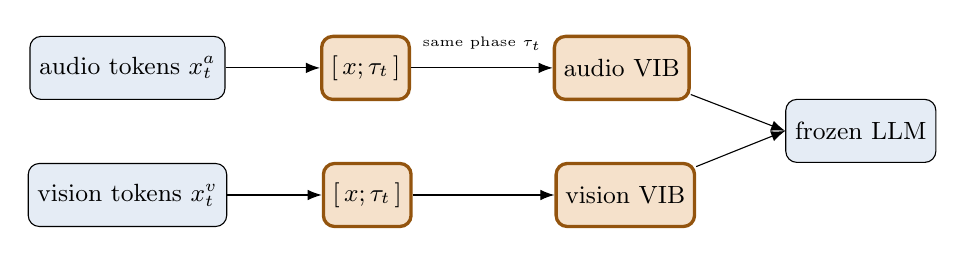
\begin{tikzpicture}[font=\small,>={Latex[length=1.8mm]},node distance=3mm and 6mm,
  trn/.style={draw,very thick,rounded corners,fill=trn!22,draw=trn!70!black,minimum height=8mm,align=center},
  frzs/.style={draw,rounded corners,fill=frz!12,minimum height=8mm,align=center}]
  \node[frzs] (a) {audio tokens $x^a_t$};
  \node[frzs,below=8mm of a] (v) {vision tokens $x^v_t$};
  \node[trn,right=12mm of a] (ca) {$[\,x;\tau_t\,]$};
  \node[trn,right=12mm of v] (cv) {$[\,x;\tau_t\,]$};
  \node[trn,right=18mm of ca] (ba) {audio VIB};
  \node[trn,right=18mm of cv] (bv) {vision VIB};
  \node[frzs,right=12mm of ba,yshift=-8mm] (llm) {frozen LLM};
  \draw[->] (a)--(ca); \draw[->] (v)--(cv);
  \draw[->] (ca)--node[above,yshift=1mm]{\tiny same phase $\tau_t$}(ba); \draw[->] (cv)--(bv);
  \draw[->] (ba)--(llm.west); \draw[->] (bv)--(llm.west);
\end{tikzpicture}
\caption{Proposed temporal extension: a shared clock feature $\tau_t$ is concatenated onto both
streams before the bottleneck, so that audio at time $t$ and a video frame at $t+\Delta$ differ in
their encodings.}
\label{fig:temporal-ext}
\end{figure}

As a controlled test of the representability hypothesis implied by Section~\ref{sec:temporal-failure}
-- namely, that misalignment is not just \emph{unused} but not even \emph{representable} by the
current bottleneck -- a shared clock feature is added to both modality streams before the bottleneck:
\[
\tilde x_t = \big[\,x_t;\ \sin(2\pi t/T),\ \cos(2\pi t/T)\,\big], \qquad h = \mathrm{GELU}(W_e\,\tilde x_t).
\]
In the formulation of Section~\ref{sec:arch}, the bottleneck receives each token without any
positional information, so audio and video at different, misaligned times are indistinguishable to
it in principle, not merely in practice. A shared phase $\tau_t$ across both streams
(Figure~\ref{fig:temporal-ext}) makes misalignment representable for the first time: audio at time
$t$ and a video frame at $t+\Delta$ now differ in their encodings purely because of the phase term,
independent of their content. At the 2\,fps frame rate used throughout this work, the frame interval
of 0.5 seconds bounds the smallest displacement this representation could possibly resolve.
$W_{\text{out}}$ remains zero-initialized, so the extension preserves the identity-at-initialization
property established in Section~\ref{sec:arch}. This extension was implemented and training was under
way at the time of writing. Given that the frozen backbone is at chance even at the largest,
most resolvable displacement tested (Section~\ref{sec:temporal-failure}), limited benefit is expected
from this change alone; the run is retained and reported as a controlled test of the representability
hypothesis, not as an anticipated improvement, in keeping with this report's commitment to
distinguishing measured results from expectations.

\clearpage
% ================================================================================================
\section{Ablations and Negative Results}
\label{sec:ablation}

\subsection{Placement of the Bottleneck}
\label{sec:placement}

\begin{figure}[h]
\centering
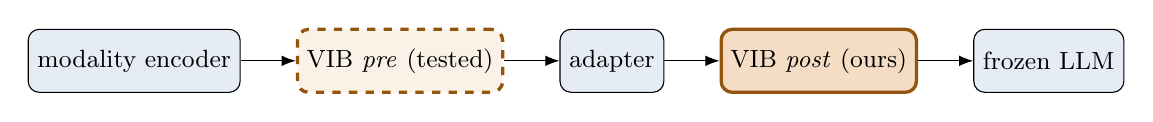
\begin{tikzpicture}[font=\small,>={Latex[length=1.8mm]},node distance=3mm and 7mm,
  frzs/.style={draw,rounded corners,fill=frz!12,minimum height=8mm,align=center},
  vibs/.style={draw,very thick,rounded corners,fill=trn!25,draw=trn!70!black,minimum height=8mm,align=center},
  vibd/.style={draw,very thick,dashed,rounded corners,fill=trn!10,draw=trn!70!black,minimum height=8mm,align=center}]
  \node[frzs] (enc) {modality encoder};
  \node[vibd,right=of enc] (pre) {VIB \emph{pre} (tested)};
  \node[frzs,right=of pre] (ad) {adapter};
  \node[vibs,right=of ad] (post) {VIB \emph{post} (ours)};
  \node[frzs,right=of post] (llm) {frozen LLM};
  \draw[->] (enc)--(pre); \draw[->] (pre)--(ad); \draw[->] (ad)--(post); \draw[->] (post)--(llm);
\end{tikzpicture}
\caption{The two placements considered for the bottleneck: applied to the modality adapter's raw
input features (pre) or to its output, in the LLM's embedding space (post, used throughout this
report).}
\label{fig:placement}
\end{figure}

The bottleneck used throughout this report is applied to the modality adapter's \emph{output}, in the
LLM's own embedding space. The alternative -- applying it to the adapter's \emph{input}, on the raw
encoder features -- was also implemented and tested (Figure~\ref{fig:placement}). The two placements
produce comparable AVHBench accuracy, so the choice between them is not decisive for performance.
This work retains the post-adapter placement for a practical reason rather than an accuracy reason:
it uses a single attachment width, equal to the LLM's hidden size, on every backbone studied, whereas
the pre-adapter variant requires a distinct attachment width for each modality and each backbone,
which complicates the four-backbone comparison of Section~\ref{sec:backbones}. The pre-adapter
attachment remains implemented in the codebase as an option (\texttt{--pre-adapter}); its
numerical results from the earlier comparison are not present in the current results directory and
are therefore not tabulated in this report.

\subsection{Negative Results}
\label{sec:negative}

\begin{table}[h]
\centering
\small
\renewcommand{\arraystretch}{1.4}
\begin{tabular}{p{3.3cm}p{5.6cm}p{4.9cm}}
\toprule
Tried & Failure & Lesson \\
\midrule
Standard DPO on swap pairs & Collapse to a constant response (PA $0.95\!\to\!0.10$) & Motivated the two rails \\
GRPO on low-difficulty items & Zero advantage on $\sim$2/3 of steps & Unanimous rewards give no gradient \\
Query-conditioned gate $g(q)$ & Remained $>0.4$ throughout & Modulation preferred to routing \\
``59\% of vision rewritten'' & Not supported by parameter inspection & Claim withdrawn \\
LoRA at identical attach points & $+2.8$ vs.\ $+5.1$; HR below base & Residual form matters, not capacity \\
\bottomrule
\end{tabular}
\caption{Negative results from this project, reported for completeness. Several directly informed
the final design described in Section~\ref{sec:method}.}
\label{tab:negative}
\end{table}

Table~\ref{tab:negative} records five results from this project that did not survive contact with
data, several of which directly shaped the method described in Section~\ref{sec:method}. Standard DPO
on the constructed swap pairs, discussed at length in Section~\ref{sec:dpo-fails}, is included here
alongside four further attempts. Group Relative Policy Optimization (GRPO; Shao et al., 2024) was
tried as an alternative to the preference-pair formulation, using the low-difficulty items in the
constructed training data as a reward signal; it produced zero policy-gradient advantage on roughly
two-thirds of training steps, because items the model already answers correctly with high confidence
give every sampled response the same (maximal) reward, leaving no contrast for the gradient estimator
to exploit. Reusing the FiLM gate $g(q)$ as a hard router rather than a continuous modulation signal
was tried directly; the gate never fell below 0.4 in practice regardless of this framing, which is why
Section~\ref{sec:params} interprets it as continuous modulation rather than discrete routing. An
earlier, stronger version of the parameter analysis in Section~\ref{sec:params} claimed that 59\% of
the vision stream was rewritten while the audio module was inactive; this claim did not survive
direct inspection of the trained parameters and was withdrawn, and is recorded here a second time in
the interest of a transparent account of what was and was not ultimately supported by evidence.
Finally, the LoRA comparison at identical attachment points is the cleanest control available in this
work for isolating the effect of the adapter's specific architectural form: with the same
attachment points, the same training data, and the same anchored objective, a LoRA-style low-rank
weight edit (Hu et al., 2022) reaches $+2.8$ points against FiLM's $+5.1$, with hallucination
resistance falling \emph{below} the frozen baseline. This indicates that the zero-initialized,
stochastic residual form of the bottleneck adapter -- not simply the presence of a small number of
trainable parameters -- is responsible for a meaningful share of the improvement reported in
Section~\ref{sec:results}.

\clearpage
% ================================================================================================
\section{Discussion}
\label{sec:discussion}

\subsection{Limitations}
\label{sec:limitations}

Three categories of limitation are recorded here explicitly, so that the scope of the claims made in
this report is unambiguous.

\textbf{Single seed.} Every result reported in Section~\ref{sec:results} and
Section~\ref{sec:generalization} comes from a single training run per configuration. The confidence
intervals reported in Table~\ref{tab:significance} reflect uncertainty from item sampling on a fixed
model only; they do not capture variation that would arise from retraining with a different random
seed. A multi-seed variance study, a sweep over the compression coefficient $\beta_{kl}$, an ablation
isolating the contribution of each term in the VIB-ingredient list, and a data-scaling curve were all
identified as valuable follow-up experiments during this project but are not included here for want
of the additional compute and time such a study would require; they are named explicitly rather than
silently omitted.

\textbf{Scope of the improvement.} Section~\ref{sec:generalization} shows that the method's benefit
is conditional on the frozen backbone already carrying usable but under-exploited audio information;
where that precondition does not hold (VideoLLaMA2, temporal alignment on Qwen3-Omni), the method
does not help. Section~\ref{sec:capability} shows a small, consistently negative, though not
statistically significant, cost on two out-of-distribution capability benchmarks. Both findings
should be read as bounding the applicability of the method, not as separate weaknesses of the specific
implementation studied here.

\textbf{Work in progress at the time of writing.} Training and evaluation of the adapter on MiniCPM-O
2.6 (Section~\ref{sec:minicpm}) had not completed; the video-substitution and temporal-displacement
training variants referenced in Section~\ref{sec:temporal-ext} were trained but not yet evaluated;
and the CMM evaluation for the cross-attention baseline of Table~\ref{tab:main-results} was still
running. These are reported as open items rather than results, consistent with the provenance
standard applied throughout this report: every number given here is either measured under this
work's own protocol or drawn from a cited publication, and nothing is estimated or extrapolated to
fill a gap.

\subsection{Reproducibility}
\label{sec:reproducibility}

The codebase developed during this internship comprises four model wrappers (one per backbone
studied), five benchmark runners, four training variants, two baseline implementations, and three
analysis probes, totalling approximately 10,000 lines of code, 23 cluster job scripts, and seven test
suites. Every table and figure in this report is produced by a single, dedicated script, so that any
number reported here can be traced back to the exact procedure that produced it. Beyond the protocol
choices already discussed in Section~\ref{sec:protocol} -- frame rate, prompts, answer format, and
decoding parameters, all fixed and logged -- checkpoint selection is always performed on a validation
half disjoint from the reported evaluation split, and per-item predictions are stored for every
evaluation run, so that the paired statistical tests of Section~\ref{sec:significance} can be
recomputed exactly from the stored predictions rather than re-run from scratch.

\clearpage
% ================================================================================================
\section{Conclusion and Future Work}
\label{sec:conclusion}

This report has presented a parameter-efficient method for improving audio grounding in a frozen
audio--visual LLM, together with an evaluation protocol designed specifically to make the resulting
claims trustworthy. The central result is that a zero-initialized variational bottleneck adapter,
under 0.5\% of backbone parameters, trained with an anchored preference objective on constructed
audio--visual conflicts, improves AVHBench accuracy by 5.1 points, and by 5.8 points with a
query-conditioned (FiLM) extension, both statistically significant ($p<10^{-4}$, paired), while
preserving hallucination resistance and incurring no significant cost on two independent
out-of-distribution capability controls. This result is not asserted on accuracy alone: two
independent mechanistic probes show that both variants increase the model's measured dependence on
the audio stream by a factor of 3.3 to 3.6, and a third probe shows that only the query-conditioned
variant also increases the attention allocated to audio-visual evidence, identifying two distinct
routes to a comparable improvement in accuracy.

The method's limits are established with the same standard of evidence as its successes. Across four
backbones, the achievable improvement tracks the audio information already present in the frozen
representation: substantial on Qwen3-Omni, negligible on Qwen2.5-Omni, and negative on VideoLLaMA2,
whose audio pathway was integrated post hoc. On temporal alignment, where the frozen backbone is
measured to be exactly at chance, the same training objective produces no improvement at all,
confirming that the bound observed across backbones is a property of what information the frozen
representation carries, not of the training procedure applied on top of it. Taken together, these
results support a general claim about this class of method: a small, reversible adapter can make
existing but under-used information in a frozen model \emph{usable}, but it cannot supply competence
the frozen model never had.

Future work identified during this internship falls into three categories. The most immediate is
completing the experiments already in progress at the time of writing: evaluating the adapter on
MiniCPM-O 2.6, and evaluating the video-substitution and temporal-displacement training variants that
were trained but not yet assessed (Section~\ref{sec:limitations}). The second is strengthening the
statistical claims made here with a multi-seed variance study and a systematic sweep of the
compression coefficient $\beta_{kl}$, both identified explicitly as gaps in
Section~\ref{sec:limitations}. The third is extending the temporal-alignment representability test of
Section~\ref{sec:temporal-ext} to completion and, depending on its outcome, investigating whether a
different intervention -- rather than a different input representation -- is needed to give the
frozen backbone usable temporal-alignment signal in the first place.

\clearpage
% ================================================================================================
\begin{thebibliography}{99}

\bibitem{alemi2017} Alemi, A.~A., Fischer, I., Dillon, J.~V., and Murphy, K. (2017). Deep Variational
Information Bottleneck. \emph{International Conference on Learning Representations (ICLR)}.

\bibitem{houlsby2019} Houlsby, N., Giurgiu, A., Jastrzebski, S., Morrone, B., de Laroussilhe, Q.,
Gesmundo, A., Attariyan, M., and Gelly, S. (2019). Parameter-Efficient Transfer Learning for NLP.
\emph{International Conference on Machine Learning (ICML)}.

\bibitem{hu2022} Hu, E.~J., Shen, Y., Wallis, P., Allen-Zhu, Z., Li, Y., Wang, S., Wang, L., and Chen,
W. (2022). LoRA: Low-Rank Adaptation of Large Language Models. \emph{International Conference on
Learning Representations (ICLR)}.

\bibitem{kingma2014} Kingma, D.~P.\ and Welling, M.\ (2014). Auto-Encoding Variational Bayes.
\emph{International Conference on Learning Representations (ICLR)}.

\bibitem{leng2024} Leng, S., et al.\ (2024). CMM: A Benchmark for Cross-Modal Hallucination in
Audio--Visual LLMs.

\bibitem{perez2018} Perez, E., Strub, F., de Vries, H., Dumoulin, V., and Courville, A. (2018). FiLM:
Visual Reasoning with a General Conditioning Layer. \emph{AAAI Conference on Artificial Intelligence}.

\bibitem{rafailov2023} Rafailov, R., Sharma, A., Mitchell, E., Ermon, S., Manning, C.~D., and Finn,
C.\ (2023). Direct Preference Optimization: Your Language Model Is Secretly a Reward Model.
\emph{Advances in Neural Information Processing Systems (NeurIPS)}.

\bibitem{shao2024} Shao, Z., et al.\ (2024). DeepSeekMath: Pushing the Limits of Mathematical
Reasoning in Open Language Models. (Introduces Group Relative Policy Optimization, GRPO.)

\bibitem{sungbin2025} Sung-Bin, K., et al.\ (2025). AVHBench: A Cross-Modal Hallucination Benchmark
for Audio--Visual Large Language Models. \emph{International Conference on Learning Representations
(ICLR)}.

\bibitem{tishby2000} Tishby, N., Pereira, F.~C., and Bialek, W.\ (2000). The Information Bottleneck
Method. \emph{Proceedings of the Allerton Conference on Communication, Control and Computing}.

\bibitem{wang2024} Wang, F., Zhou, W., Huang, J.-t., Xu, N., Zhang, S., Poon, H., and Chen, M.\
(2024). mDPO: Conditional Preference Optimization for Multimodal Large Language Models.

\bibitem{wen2026} Wen, Y., et al.\ (2026). arXiv:2605.16403.

\end{thebibliography}

\end{document}
